\section{音楽室}\label{sec:MUC}\index{おんがくしつ@音楽室|textbf}


ハローこんにちは!熊野寮に並みいるヘンテコスペースの中でも特にブッ飛んだ、音楽室の紹介をするぜ!

既にご存知かもしれないが、熊野寮は世にも珍しい、音楽室があるブッ飛んだ寮なのだ!!そして音楽室ユーザー全体から成る、音楽室を自分たちの手で管理、運営するブッ飛んだ団体が我々
\vskip\baselineskip

{\huge MUC : \textit{Music room Users' Conference}}\\
なのである!\index{MUC@MUC(音楽室利用者会議)}\index{おんがくしつりようしゃかいぎ@音楽室利用者会議|see{MUC}}

音楽室といっても学校の音楽室のようなものでなく、アンプやキーボード、ドラムなどのバンド用の機材がそろったブッ飛んだ空間だ。バンド演奏を中心に使われているが、歌の練習、ダンスの練習にも使われている。つまりは実質フリースペース!ついでに利用料もフリー!

また、その発表の場として寮内で開かれるブッ飛んだライブに出ることもできるぞ!ライブはほぼ月1でやってるから最早やりすぎって感じだ!毎回ライブでは寮内の音楽好きが集まってめちゃめちゃ盛り上がるぜ!出演バンドは例えばアジカンやKing Gnuなどロックのコピバンが多いな!たくさんライブに出てブッ飛んだ時間を作ろう!

じゃあMUCって具体的に何すんのかな?それは大きく分けて3つある。一つは音楽室機材のブッ飛んだメンテ、管理。一つはライブの準備。そして毎週月曜のブッ飛んだミーティングだ。いずれも詳しく書くことは控えておくが、たくさんの人と交流できるブッ飛んだ仕事だ!音楽機材に強くなれたりもするぜ!

音楽室はどうやったら使えるようになるのかって?それは毎週月曜日の21:30からやってるMUC会議に出ればOKだ!ちなみに音楽室は寮生じゃなくても会議に来るだけで使えるぜ!音楽好きな奴はMUC会議に来てくれよな!

バンドでライブ\index{らいぶ@ライブ|textbf}がしたい?ダンスでクールに決めたい?うんうん!大いに歓迎しよう。ちょっとだけ興味あるけど… うんうん!君も大歓迎だ!ブッ飛んだ紹介は以上だ!諸君!MUCで会おうぜ!





\begin{figure}[bh]
	\centering
	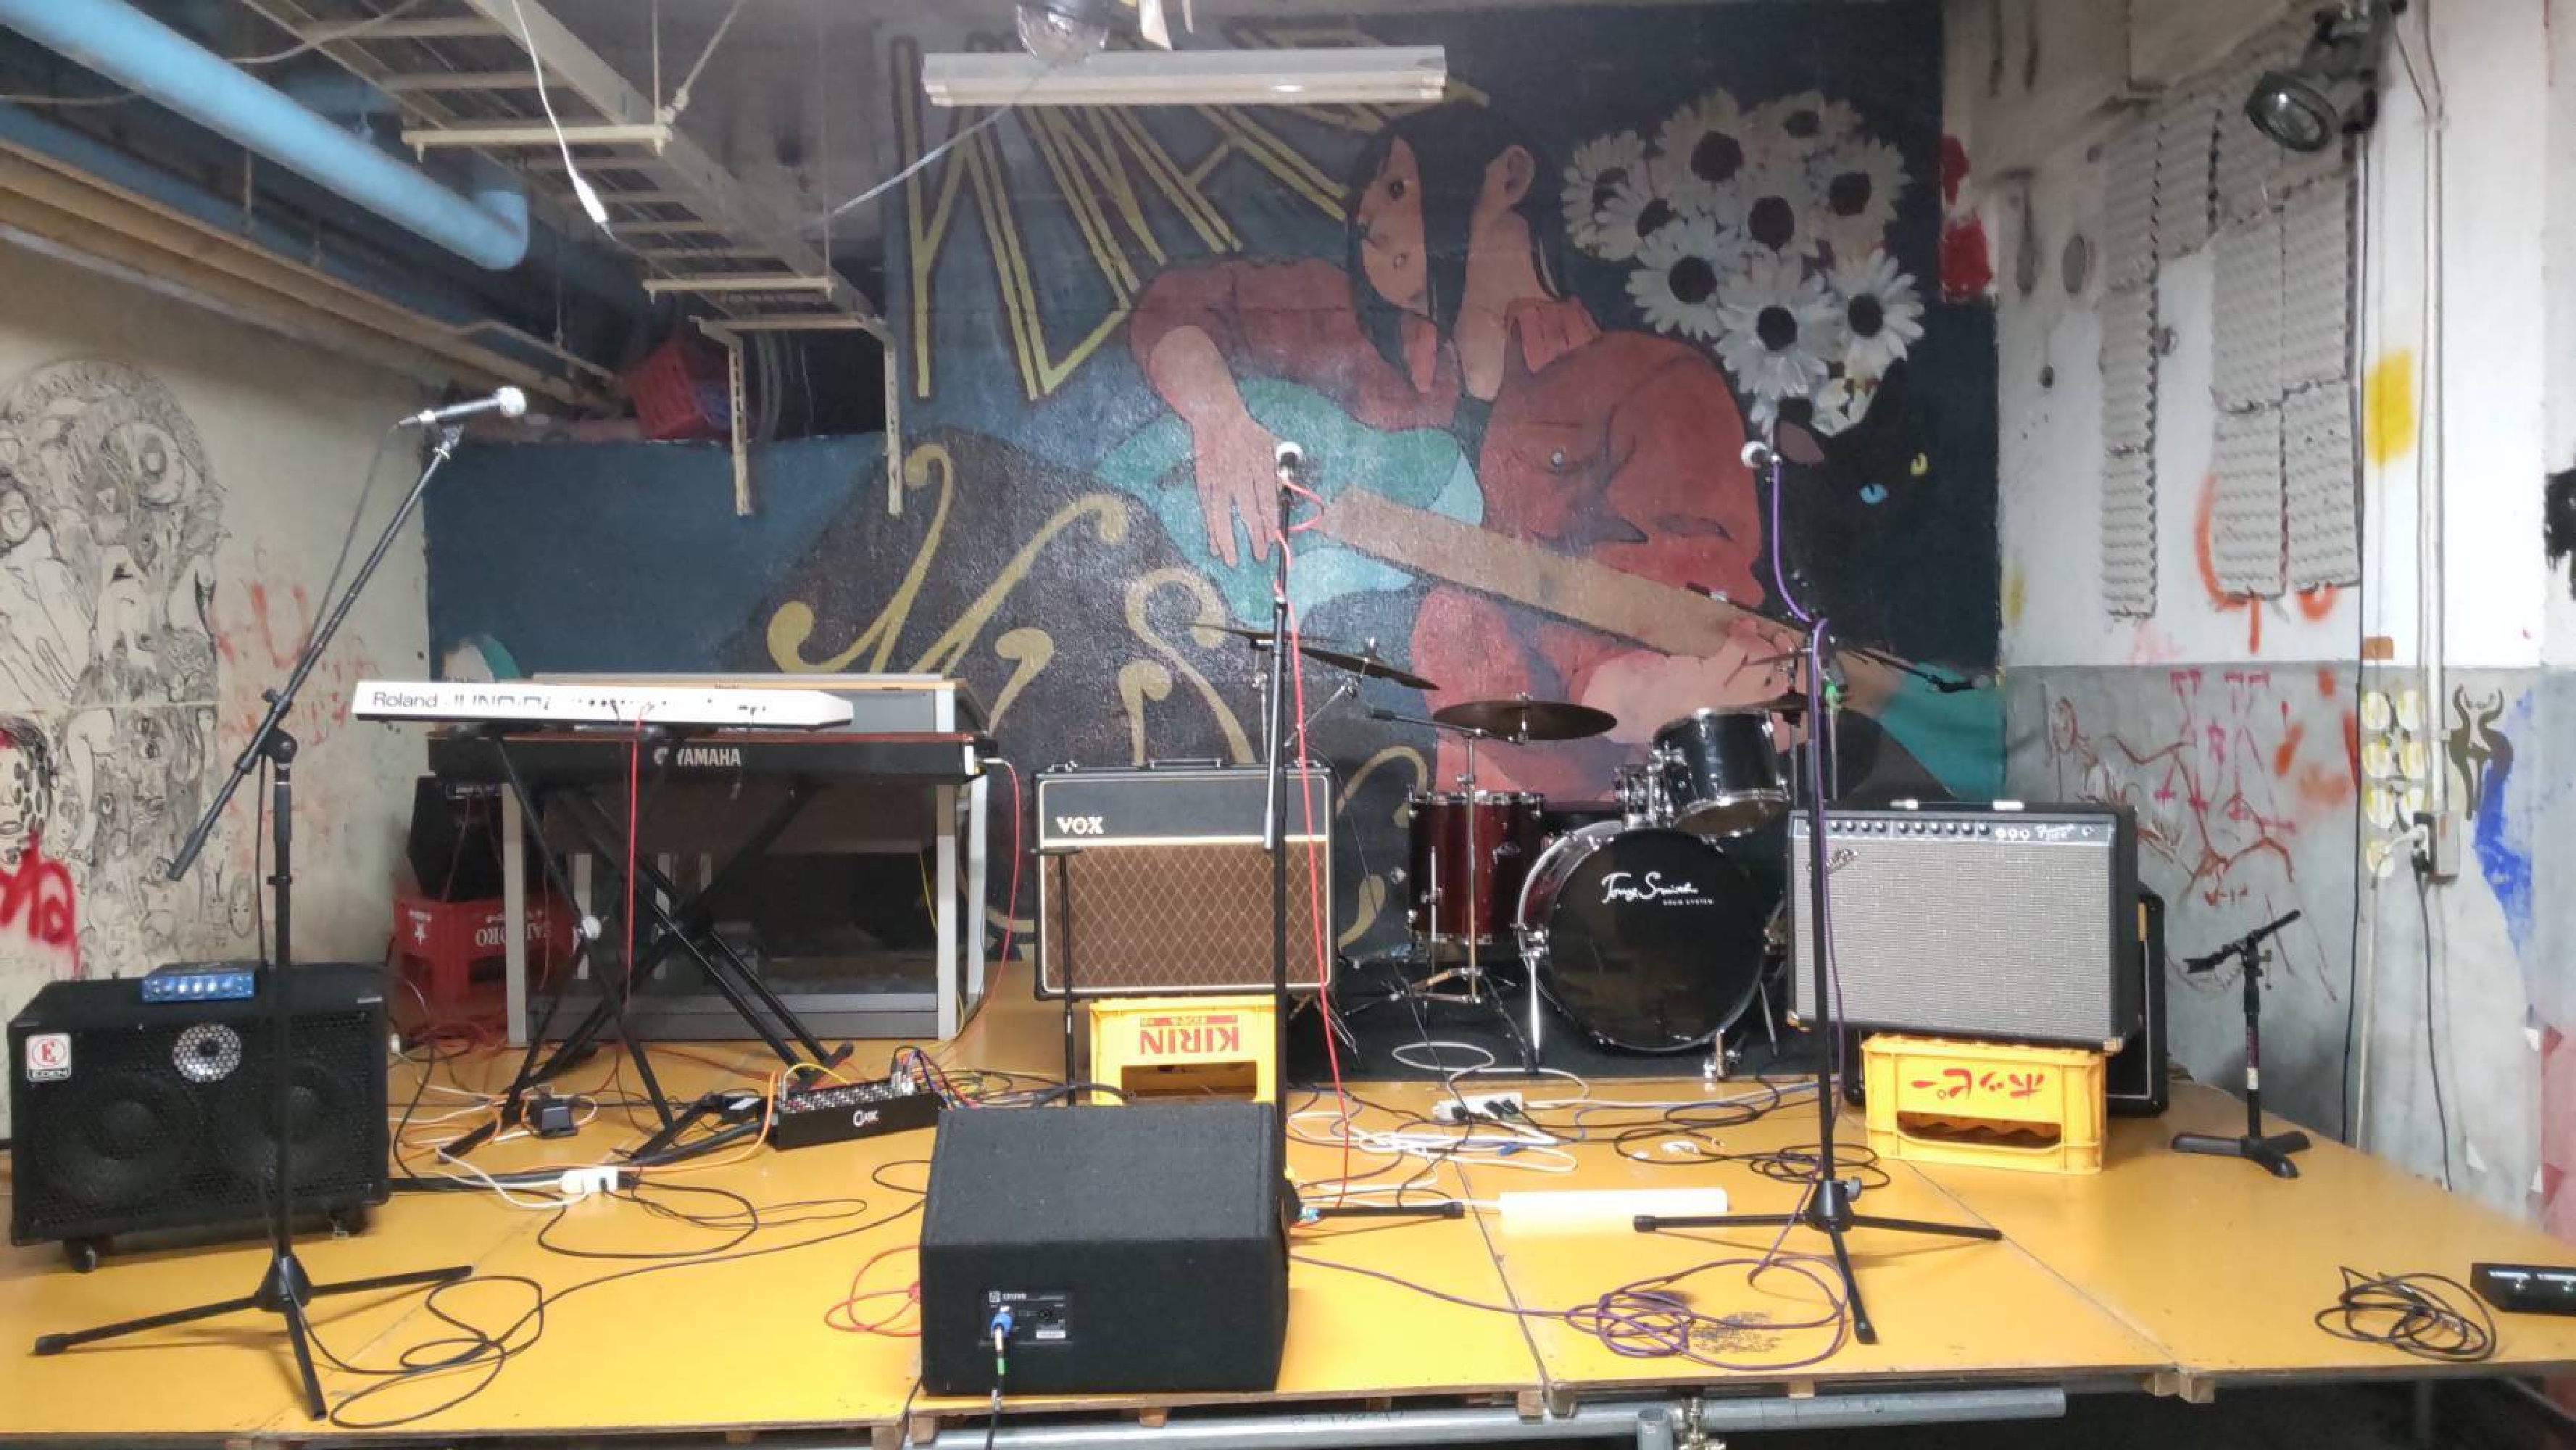
\includegraphics[width=16cm]{gazo/music_room.pdf}
\end{figure}